\chapter{Полугруппы и полурешетки}

\begin{my_def}
Бинарная операция~$*$ на множестве~$S$ --- это функция
$$f: S^2 \rightarrow S.$$
Значение бинарной операции для $x, y \in S$ обозначают~$x * y = f(x, y)$.
\end{my_def}


\begin{my_def}
Пусть~$*$ --- бинарная операция определённая на множестве~$S$, а
$x, y, z \in S$~--- произвольные элементы множества $S$. Тогда если
выполняется равенство
$$x * y = y * x,$$
то операция~$*$ называется коммутативной.
Если выполняется
$$
x * (y * z) = (x * y) * z,
$$
то операция~$*$ называется ассоциативной.
Если выполняется
$$
x * x = x,
$$
то операция~$*$ называется идемпотентной.
\end{my_def}


\begin{my_def}
Полугруппа --- множество с заданной на нём ассоциативной бинарной операцией~$(S,*)$.
\end{my_def}


\begin{my_def}
Полурешетка --- это полугруппа, бинарная операция которой коммутативна и
идемпотентна.
\end{my_def}

Для полурешетки можно определить частичный порядок

$$x \leq y \Leftrightarrow x*y=x.$$

\section{Таблица Кэли}

Таблица Кэли --- таблица, которая описывает структуру конечных алгебраических систем путём расположения результатов операции в таблице, напоминающей таблицу умножения. Названа в честь английского математика Артура Кэли. Таблица имеет важное значение в дискретной математике, в частности, в теории групп. Таблица позволяет выяснить некоторые свойства группы, например, является ли группа абелевой, найти центр группы и обратные элементы элементов группы.

В высшей алгебре таблицы Кэли могут также использоваться для определения бинарных операций в полях, кольцах и других алгебраических структурах.

Простой пример таблицы Кэли для группы ${1, -1}$ с обычным умножением:

\begin{center}
\begin{tabular}{ |g|c|c| }
\hline
\rowcolor{Gray}
$\times$ & 1 & -1 \\
\hline
1 & 1 & -1 \\
\hline
-1 & -1 & 1 \\
\hline
\end{tabular}
\end{center}

\section{Граф полурешетки}

Каждой полурешетке можно сопоставить ориентированный граф. Этот граф можно построить следующим образом.

Пусть полурештка состоит из элементов $0, 1, \ldots, n-1$ и задана таблицей Кэли.

Шаг 1. Находим корень дерева $root$:
$$
root = 0 \cdot 1 \ldots \cdot (n-1).
$$

Шаг 2. Находим смежные с $root$ вершины. Для этого перебираем все элементы $x$ полурешётки и отбираем те из них, которые удовлетворяют условиям: $x \neq root$ , $x \cdot root = root$, не существует элемента $z$, такого, что $z \neq x$, $z \neq root$, $z \cdot root = root$, $z \cdot x = z$. Это и будут смежные с $root$ вершины.

Шаг 3. Аналогично находим смежные вершины с найденными и т.д. пока не исчерпаются все вершины.

\section{Примеры}

Рассмотрим примеры полурешеток с такой таблицей Кэли:

\begin{center}
\begin{tabular}{ |g|c|c|c| } \hline
\rowcolor{Gray}
$\times$ & 0 & 1 & 2 \\ \hline
0 & 0 & 0 & 0 \\ \hline
1 & 0 & 1 & 1 \\ \hline
2 & 0 & 1 & 2\\ \hline
\end{tabular}
\end{center}

Граф, который будет ей будет соответствовать:

\begin{center}
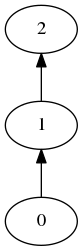
\includegraphics[height=200px]{dot_graphs/ex1.dot.png}
\end{center}
